 \documentclass[USenglish]{article}
\usepackage{babel}[USenglish]
\usepackage[utf8]{inputenc}%(only for the pdftex engine)
%\RequirePackage[no-math]{fontspec}[2017/03/31]%(only for the luatex or the xetex engine)
\usepackage[small]{dgruyter}
\usepackage{wrapfig}
\usepackage{booktabs}
\captionsetup{justification=centering}
\usepackage{subcaption} 
\usepackage{microtype}
\usepackage{lmodern}% http://ctan.org/pkg/lm
%\usepackage[backend=bibtex]{biblatex}

\begin{document}

  % \articletype{chapter}

  \author*[1]{Melvin Wevers}
  %\author[2]{...}
  %\author[1]{Melvin Wevers} 
  \runningauthor{Wevers}
  \affil[1]{DHLAB - KNAW Humanities Cluster}
  %\affil[2]{...}
  \title{Mining Historical Advertisements in Digitized Newspapers}
  \runningtitle{Mining Historical Ads}
  %\subtitle{}
  \abstract{Historians have turned their focus to newspaper articles as a proxy of public discourse, while advertisements remain an understudied source of digitized information. This paper focuses on how historians can use computational methods to work with extensive collections of advertisements. First, this chapter analyzes metadata to understand better the different types of advertisements, which come in a wide range of shapes and sizes. Information on the size and position of advertisements can help to construct particular subsets of advertisements. Second, this chapter describes how textual information can be extracted from historical advertisements that can subsequently be used for historical analysis of trends and particularities. For this purpose, we present a case study based on cigarette advertisements.}
  \keywords{historical advertisements, text mining, digitized newspapers, digital history}
  %\classification[PACS]{...}
  %\communicated{...}
  %\dedication{...}
  \received{...}
  \accepted{...}
  \journalname{...}
  \journalyear{...}
  \journalvolume{..}
  \journalissue{..}
  \startpage{1}
  \aop
  \DOI{...}

\maketitle

\section{Introduction}

In recent years, we have seen an explosive growth of digitized historical newspapers. Innovations in natural language processing have extended the possibilities for historians to extract information from large corpora of digitized historical texts. National libraries and project such as impresso, Newseye, and Oceanic Exchanges offer access to digitized archives of historical newspapers.\footnote{\url{https://impresso-project.ch/}, \url{https://www.newseye.eu/}, \url{https://oceanicexchanges.org/}}

For many historians, newspapers provide a longitudinal understanding of public discourse~\cite{postman_amusing_2005,vree_nederlandse_1989}. Newspapers are not the only gateway to public discourse, since they do not capture public discourse in its entirety. In its function as a proxy, a newspaper operates as a transceiver; it is both the producer and the messenger of public discourse~\cite[17-18]{schudson_power_1982}. On a surface level, newspapers inform us about the views of journalists and people that were interviewed by these journalists. However, as Margaret Marshall claims, scholars can also uncover the ``values, assumptions, and concerns, and ways of thinking that were a part of the public discourse of that time'' by analyzing ``the arguments, language, the discourse practices that inhabit the pages of public magazines, newspapers, and early professional journals~\cite[8]{marshall_contesting_1995}.'' With easier access to and increased availability of newspaper repositories, studies of the representation of ideas, values, and practices in public discourse gained traction~\cite{van_eijnatten_eurocentric_2019,daems_workers_2019}. 

Even though newspapers contain a considerable amount of advertisements, these remain an understudied source in computational studies of public discourse. This is surprising since advertisements are rich and varied carriers of information of the past. In his seminal work \textit{Advertising the American Dream}, Roland Marchand argues that adverts offer a lens on the past and provide ``insight into the ideals and aspirations of past realities [...] they show the state of technology, the social functions of products, and provide information on the society in which a product was sold~\cite{marchand_advertising_1985}.'' Others point out that even though adverts provide perspectives on the past, this is a distorted one, as the content of ads is driven by commercial interest~\cite{fox_mirror_1997}. 
%
Marchand acknowledges this criticism and conceptualizes advertisements as distorted mirrors. He argues that despite the primary function of advertisements to sell products, they still communicated social and cultural values, albeit in a somewhat distorted manner~\cite{marchand_advertising_1985,lears_fables_1994}. 

Moreover, one could argue that for ads to be successful, they needed to resonate with their audience. As such, they had to be reflective of aspects of public discourse. Still, it is crucial to remain critical of the skewed representation of ideas and values in historical advertisements. 

Advertisements are a fascinating and complex historical source, partly because of their multi-modal nature; they contain both visual and textual content. Since there often is an interplay between the visual and textual material, an analysis of only the textual content is somewhat limited. In recent years, advances in computer vision research have provided methods to examine digitized visual material at scale. While the use of computer vision is rapidly evolving and already offers promising methods of analysis, it falls outside of this chapter's focus~\cite{wevers_visual_2020,arnold_distant_2019,Bergel_2015}. In this chapter, the topic of concern is the  analysis of metadata and textual content.

The ability to extract information from large numbers of advertisements, both synchronically and diachronically, allows scholars to study cultural expressions on a macro-scale. However, the use of computational methods can also offer fine-grained contextualizations of specific expressions. More often than not, historical interpretations drawn from advertisements are based on a small selection of ads, which might lead to cherry-picking. The ability to chart trends over time makes it possible to model whether findings in smaller subsets can be generalized, or whether specific expressions deviate from general patterns. On an intermediate, mesoscale, one can also more easily find variations of a single cultural expression. These insights gained with computational methods supplement existing modes of analysis. 

However, we also have to take into account that the quality of digitized historical sources is often sub-optimal, despite advances in Optical Character Recognition (OCR) software and natural language processing. It is especially challenging for OCR software to recognize text in advertisements correctly. In addition to more generic factors such as the quality of paper or the printing technique, text in advertisements is often presented in varying sizes and fonts or as part of a heavily-stylized logo. OCR software regularly turns these forms of textual content into gibberish. The suboptimal text quality makes it more challenging to study adverts than articles.

Despite these shortcomings, we can still extract meaningful information from the OCR-ed text. Given the amount of data, we can still find patterns in advertising discourse despite the noisy nature of the text. In this process, we have to be selective of the methods that we use, since their performance can be impacted in different ways by imperfect OCR~\cite{van_strien_assessing_2020,hillQuantifyingImpactDirty2019}. In addition to the OCR-ed text, we can also learn about trends in advertising from metadata on the position and size of advertisements in newspapers. We can, thus, study multiple aspects of advertisements using computational means. 

This chapter showcases how we can use computational techniques to study advertisements at scale in extensive collections of digitized newspapers. The first section shows how we can use metadata to examine trends in advertising. The second section gives examples of how text mining can be used to extract information from advertisements. This step is explained by demonstrating a case on product nationalities associated with cigarettes. In this case study, we rely on text mining to better understand changes and continuities in the associations with nationalities in advertisements for cigarettes.

\section{Metadata Analysis: Advertisements in Almost All Shapes and Sizes}

The digitization of newspapers has made it possible to study advertisements at scale using key word searches. However, not all digitized newspaper collections have segmented the articles and advertisements, presenting users with full-page scans that contain multiple document types, for example, advertisements and articles. In cases where text blocks were segmented but not classified, text classifiers can be used to identify document types~\cite{bilgin_utilizing_2018}. After training a text classifier with annotated data, the classifier could then predict metadata for unseen new data. Recently, there have been efforts to rely on computer vision to segment and classify the elements on a newspaper page (e.g. articles, tables, ads).\footnote{See, for example, Ben Lee's project \textit{Newspaper Navigator} at the Library of Congress. \url{https://github.com/LibraryOfCongress/newspaper-navigator}} 

Fortunately, Delpher, the digitized Dutch newspaper archive hosted by the National Library of the Netherlands (KB), includes segmented documents and metadata on the document type.\footnote{\url{http://www.delpher.nl}. The metadata on document type was manually added.} Access to this type of metadata  allows researchers to filter for advertisements. For the twentieth century alone, we can quickly assess that Delpher holds over thirty million advertisements in national and regional newspapers. Browsing through the results, it becomes clear that advertisements come in a wide range of shapes and sizes. We can find tiny, square-shaped advertisements;  column-shaped classifieds advertisements; and full-age spreads (see Figure~\ref{fig:classifieds} for an example of a column of classified ads). The content and target audiences of these ads vary considerably. How can we deal with this variation, without more specific metadata information? 
\begin{wrapfigure}{r}{0.15\textwidth}
  \vspace{-10mm}
  \begin{center}
    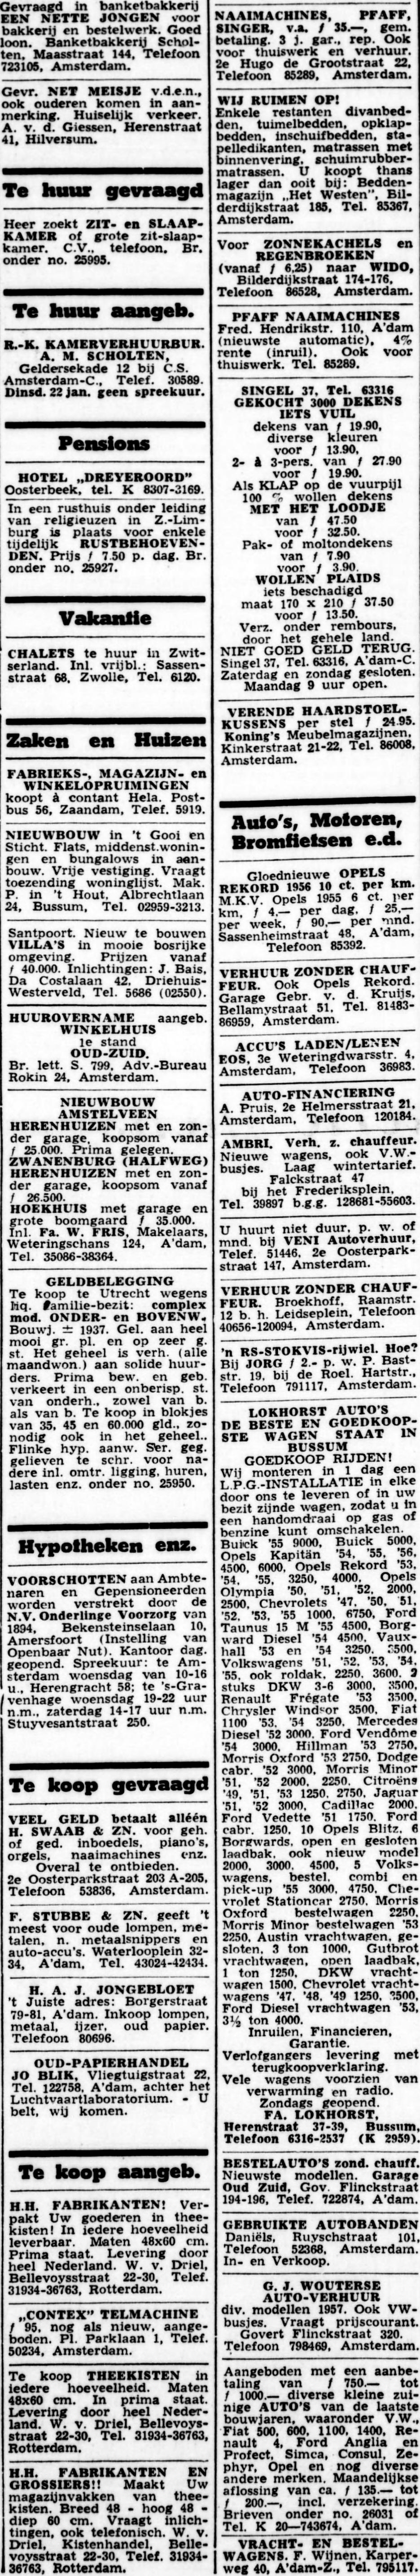
\includegraphics[height=0.40\textheight]{figures/classifieds}
  \end{center}
  \caption{Classified adverts from \textit{De Tijd}, 19 January, 1957}
  \vspace{-7mm}
  \label{fig:classifieds}
\end{wrapfigure}
%
This section shows how we can use metadata on the size and position of advertisements to cluster types of advertisements and subsequently filter out subsets. The analysis in this section is based on the metadata of the national newspaper \textit{Trouw} (1946-1995).\footnote{For most of the examples in this chapter, direct access to the metadata and newspaper data is required. Researchers can contact KB for API access to the newspapers. Code is available on: \url{https://github.com/melvinwevers/eldorado}} An initial exploratory data analysis shows that the title contains instances of bad segmentation, in which small parts of advertisements appeared as separate advertisements. To exclude these segmentation errors, we filtered out ads with a width or height smaller than 100 pixels. After removing these advertisements, \textit{Trouw} contains about 1.31 million advertisements for the period 1945-1995. From Figure~\ref{fig:ad_curve}, we can gauge that the total number of advertisements increased between 1946 and 1995, with a sudden increase in the early 1980s. Alongside this increase in the number of ads, we also see a sudden, albeit slight decrease in the size (Figure~\ref{fig:mean_size}). We plotted took the $log_{10}$ of the mean size to visualize the rate of change better. 

\begin{figure}%
  \centering
  %
  %\qquad
  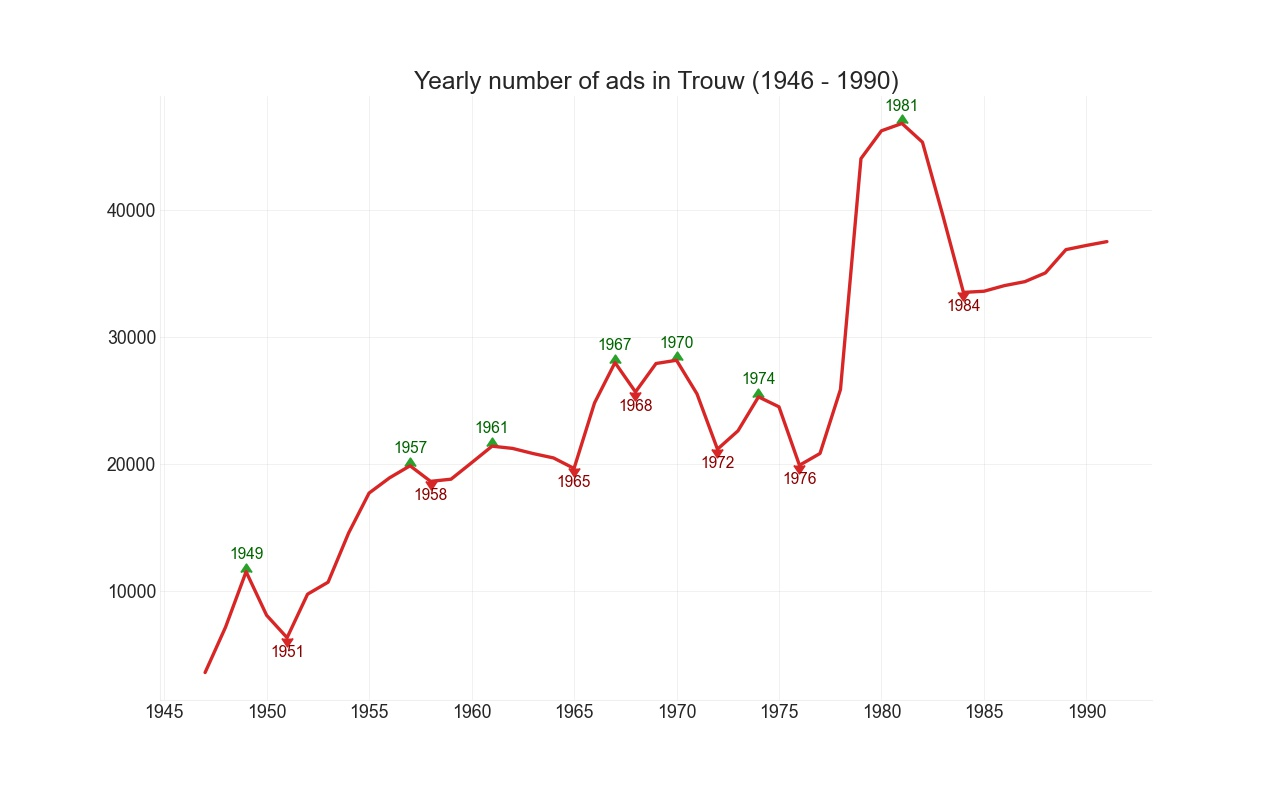
\includegraphics[width=.9\textwidth]{figures/Trouw_ad_curve}%
  \caption{Yearly number of advertisements in \textit{Trouw}. Green triangles indicate peaks and red triangle troughs.}%
  \label{fig:ad_curve}%
\end{figure}

\begin{figure}%
  \centering
  %
  %\qquad
  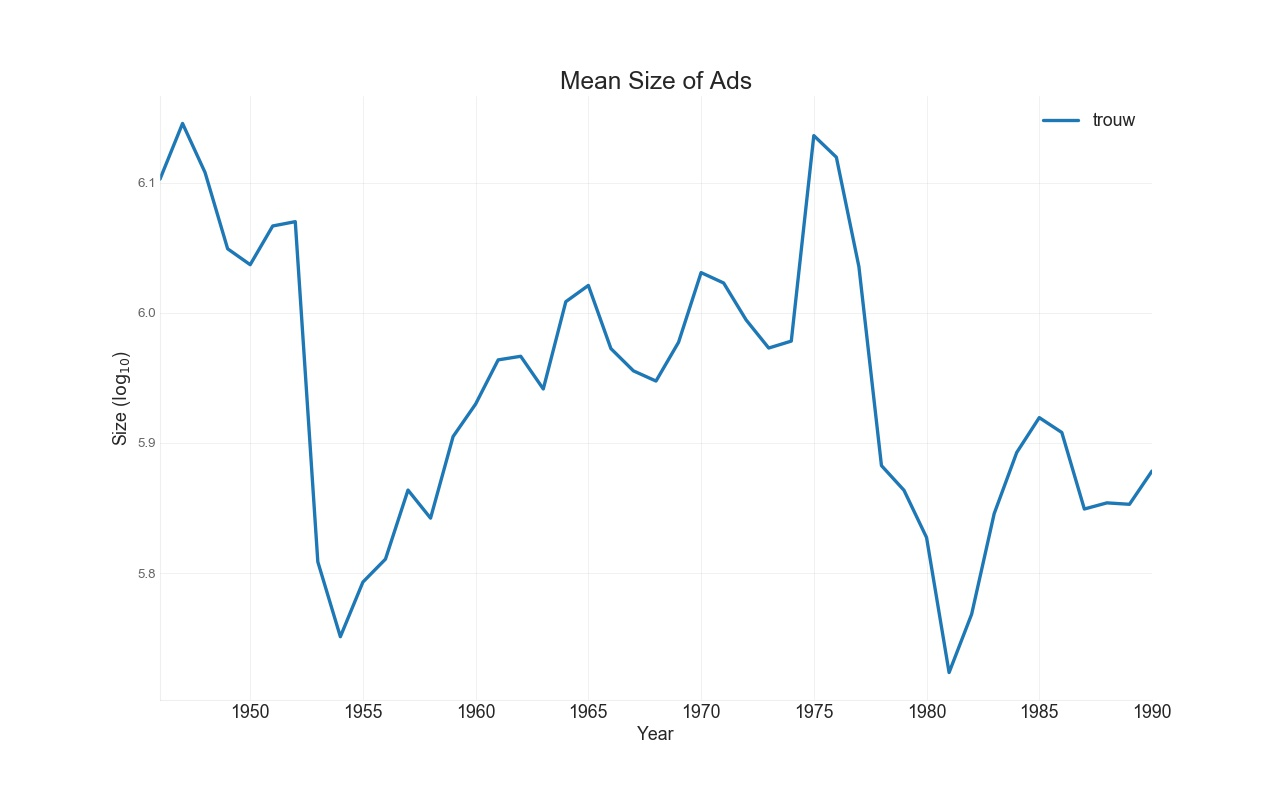
\includegraphics[width=.9\textwidth]{figures/mean_size}%
  \caption{Mean size of advertisements in \textit{Trouw}}
  \label{fig:mean_size}%
\end{figure}


In addition to their size, we can also examine where ads are positioned in the newspaper and on the individual pages. Using the width and height information of advertisements, we can create a heat map that shows which parts of the page are taken up by advertisements. There is a clear difference in pixel density between odd and even pages in \textit{Trouw} (Figure~\ref{fig:heatmapa} \& \ref{fig:heatmapb}). This can be explained by the fact that advertising on odd pages is more expensive than on even pages, as well as the common practice that new sections generally start on the odd pages. Moreover, we see that on the even pages, the upper-left corner, which is closer to the margin, is less populated than the lower-right side. 

To get a better grasp of the different groups of ads based on their 
size and their position in the newspaper, we can also apply unsupervised clustering methods, e.g. Gaussian Mixture modeling. We base this clustering on the features: width, height, and relative position of the ad in the issue. The latter indicates how close the ad is to the front page or the last page. The distribution of these features contains multiple peaks, indicative of multiple sub-distributions. To be able to capture the distributions of these subpopulations, we can use Gaussian Mixture modeling, which can estimate the parameters of these mixtures.\footnote{Scikit-Learn offers the Gaussian mixture algorithm for the estimation of a mixture model.} Compared to K-means clustering, mixture models incorporate information on the covariance structure of the data, making it possible to capture clusters with varying distributional shapes. We apply the clustering separately to even and odd pages, since there seem to be different generative principles at play, as evinced by the heat maps in Figure~\ref{fig:heatmapa} \& \ref{fig:heatmapb}. After estimating the optimal number of clusters for even and odd pages ($n$ = 8 and $n$ = 7), we fit a Gaussian Mixture model to the data.

\begin{figure}
  \centering
  \begin{subfigure}[b]{0.4\textwidth}
    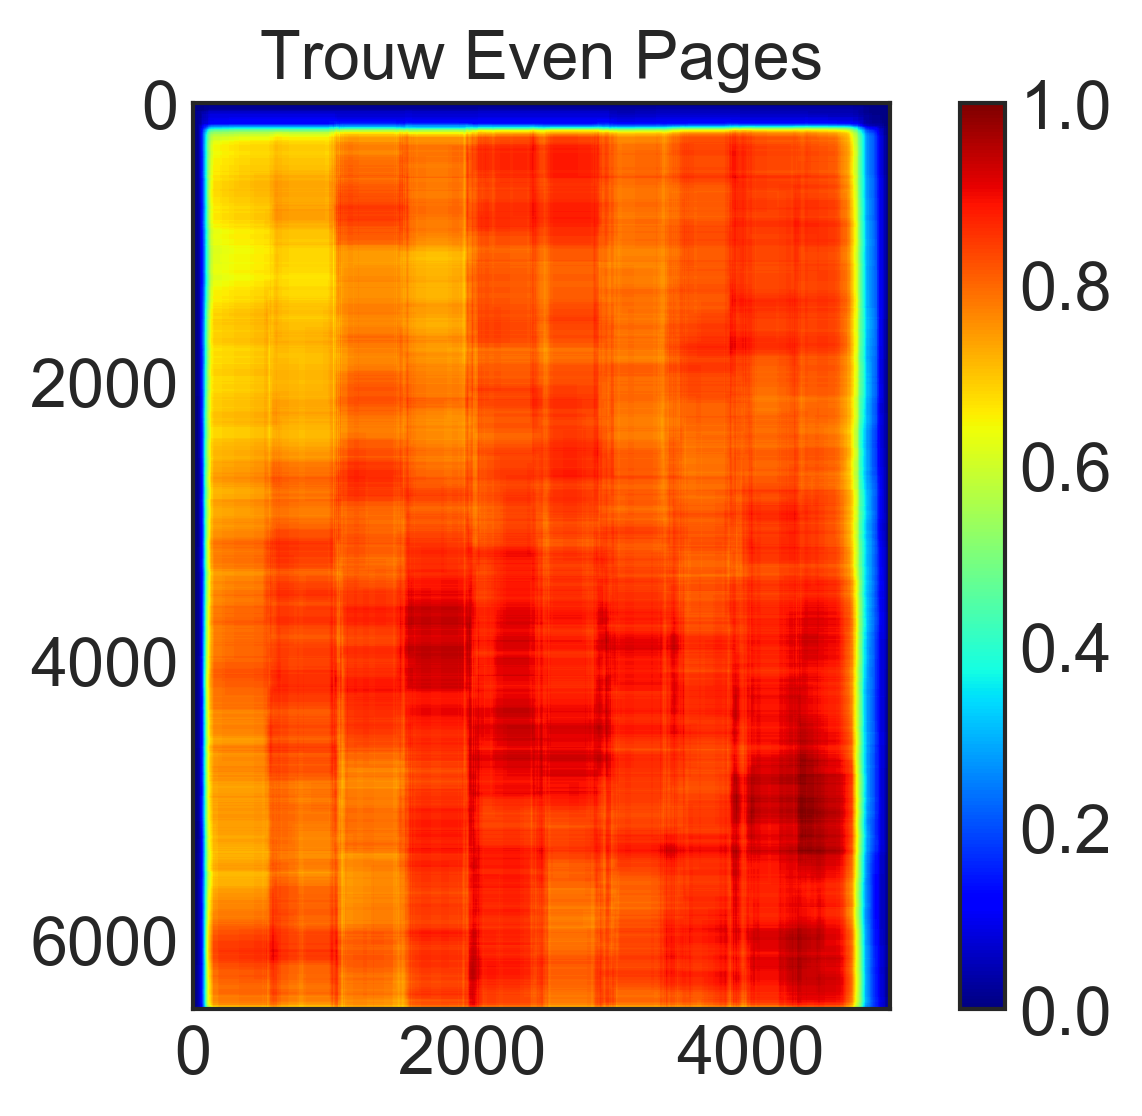
\includegraphics[width=\textwidth]{figures/Trouw_Even_Pages_heatmap}
    \caption{Pixel Density of Advertisements on Even Pages in \textit{Trouw}}
    \label{fig:heatmapa}
  \end{subfigure}
  %
  \begin{subfigure}[b]{0.4\textwidth}
    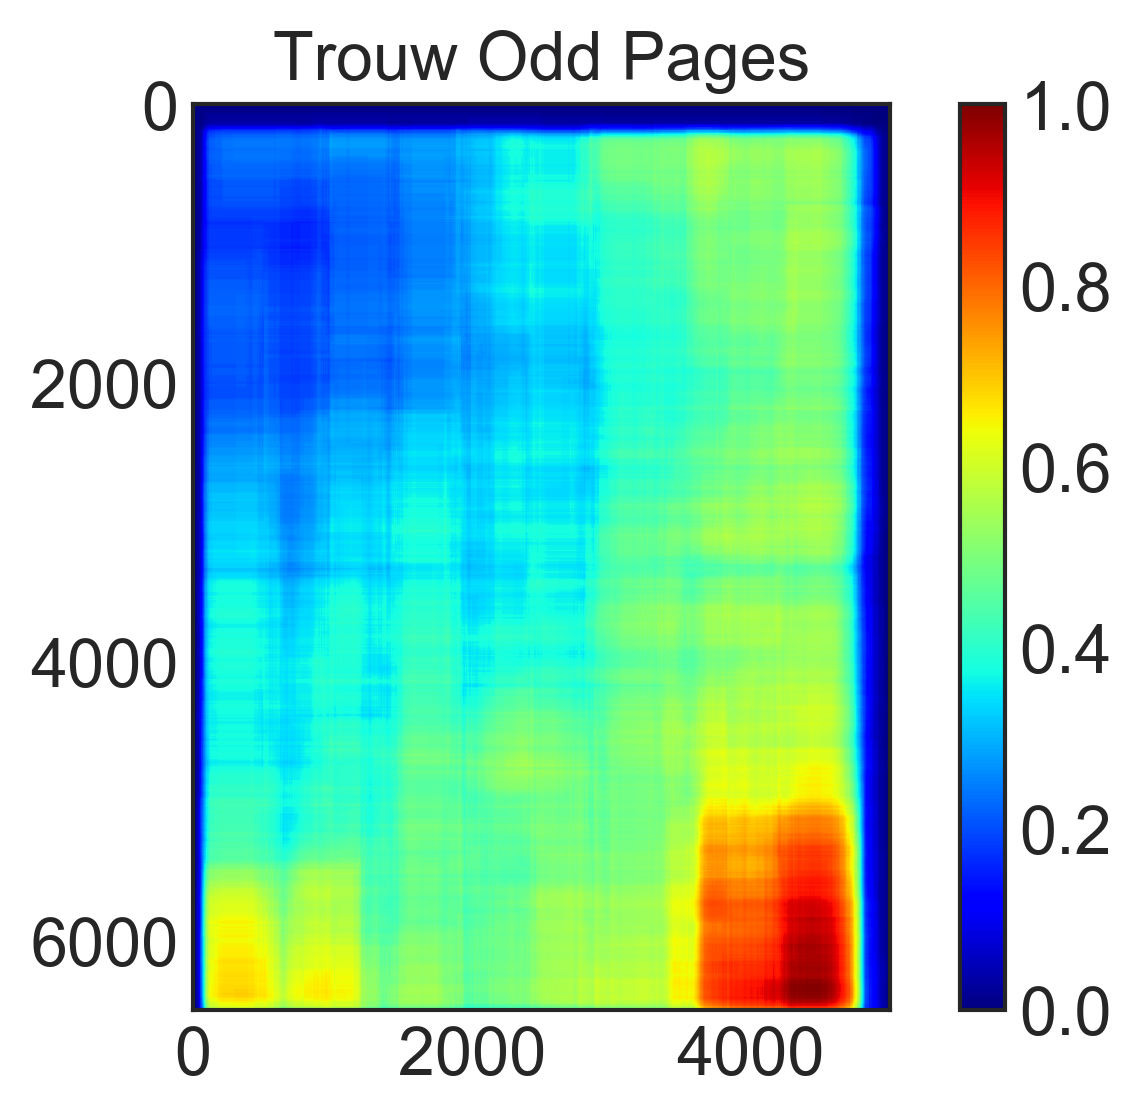
\includegraphics[width=\textwidth]{figures/Trouw_Odd_Pages_heatmap}
    \caption{Pixel Density of Advertisements on Odd Pages in \textit{Trouw}}
    \label{fig:heatmapb}
  \end{subfigure}
  \caption{Heat maps of pixel density in \textit{Trouw}}
\end{figure}



\begin{figure}
  \centering
  \begin{subfigure}[b]{0.8\textwidth}
    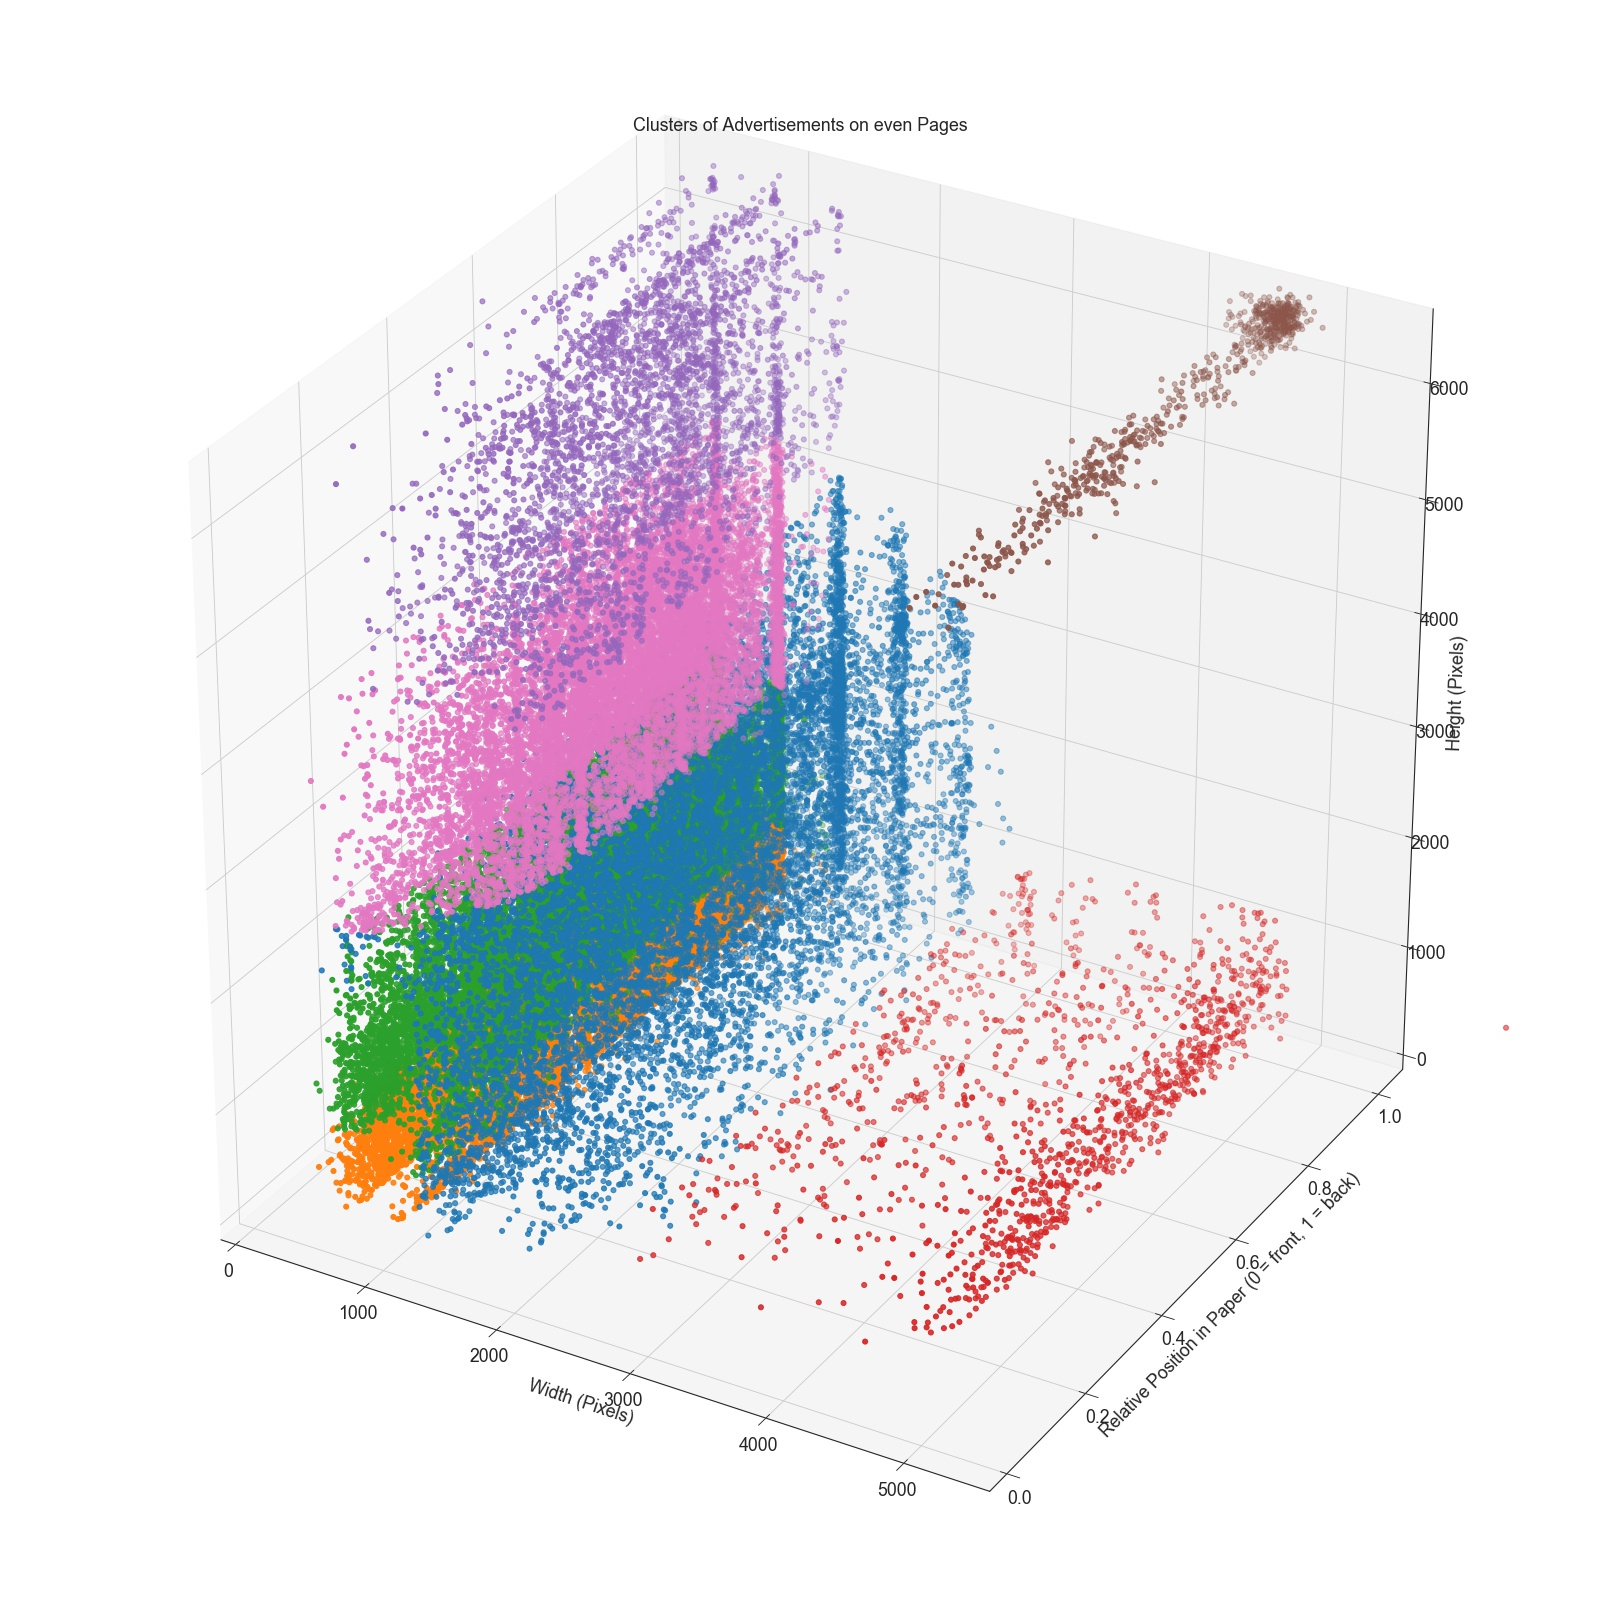
\includegraphics[width=\textwidth]{figures/even_sizes}
    \caption{Clusters of advertisement based on width, height and relative page number on even pages in \textit{Trouw}}
    \label{fig:clustera}
  \end{subfigure}
  %
  \begin{subfigure}[b]{0.8\textwidth}
    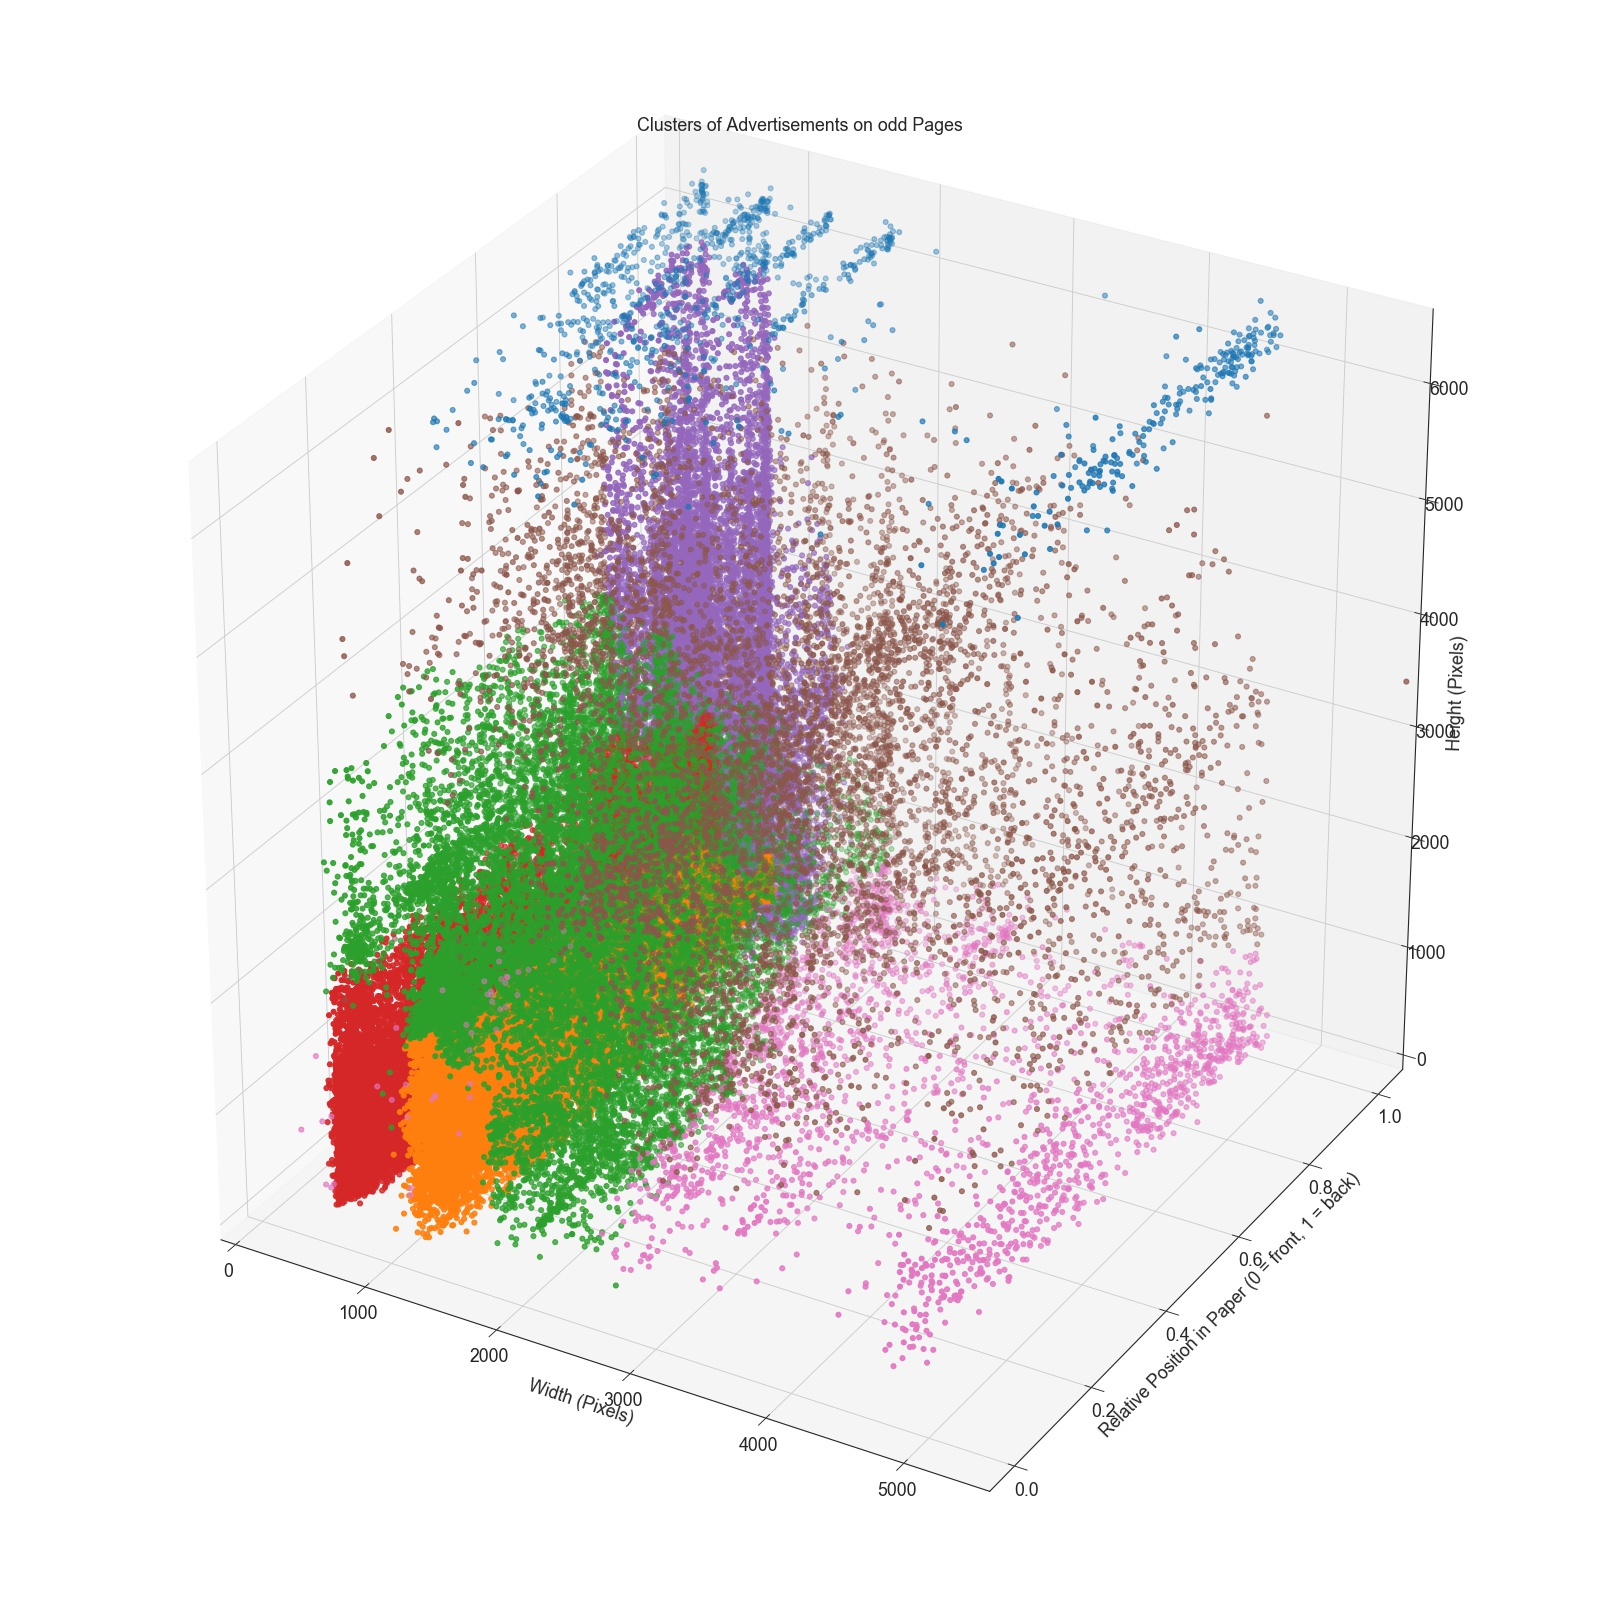
\includegraphics[width=\textwidth]{figures/odd_sizes}
    \caption{Clusters of advertisement based on width, height and relative page number on odd pages in \textit{Trouw}}
    \label{fig:clusterb}
  \end{subfigure}
  \caption{Cluster analysis of advertisements in \textit{Trouw}.
\end{figure}

The results of this clustering are presented in Figures~\ref{fig:clustera} \& ~\ref{fig:clusterb}. These plots are based on a sample of 50,000 ads from even and odd pages. We see apparent differences in size and position in the newspaper between the odd and even pages. The odd pages are less structures and lack a clear signal and show more noise, especially for ads with larger sizes. The ads on the even pages seems to be more structured. For some of these clusters, there is more variation, while others are closely clustered. A noteworthy cluster on the even pages is the brown cluster, which refers to full-page ads. 
%
We can also see that these ads appear toward the end of the newspaper. Newspapers are generally structured in columns, which is visible in the distinct structure present in the widths of advertisements (x-axis). The height of ads (y-axis) has more variance than the width, nevertheless, the algorithm distinguishes clusters based on their height. In terms of relative position, the number of advertisements increases towards the back of the newspaper (z-axis). Ads with a small width and a more considerable height, possibly classifieds ads (see Figure~\ref{fig:classifieds}, also appear toward the end of the paper. 

The information contained in these clusters can help us filter out particular subsets of advertisements. For example, maybe we are not interested in classifieds ads or tiny ads. This method can help us determine the boundaries of these ads in terms of size and position. 

We can also engineer additional features that help us refine our subsets even further. A useful feature, for instance, is character proportion, which can be calculated by dividing the number of characters by the size (width $x$ height) of the adverts. We can use this metric to filter out textual advertisements or those that predominantly consist of visual material. A similar feature is the ratio of digits to characters. This feature can be used to distinguish ads that mostly list prices of imported goods or wholesale goods, from other ads. 
%
Ostensibly, these numbers are dependent on the quality of the text extracted by Optical Character Recognition (OCR). Notwithstanding variations between newspapers and differences over time, these numbers allow us to filter particular types of advertisements. For example, we can filter out ads by inspecting particular clusters in the distribution of the character proportion. This form of exploratory data analysis can, for example, help to quickly filter out specific types of advertisements, such as classifieds. These advertisements are characterized by a higher than average height and smaller width, as well as a higher character proportion. We could also combine this metadata information with keyword search to further filter out types of ads for specific products. 

In this section, we have demonstrated a possible approach to using metadata to learn more about the structure of advertisements in historical newspapers. There are many more directions to explore. However, this section underscores that metadata should not be overlooked and can be used in conjunction with text analysis to guide further analysis. 

\section{Text Mining Advertisements}
In this section, we show how we can extract textual information from historical advertisements, and how this textual information can be used for the analysis of trends and particularities. More specifically, we present a case study on the advertised nationalities of cigarettes. We constructed our corpus of cigarette advertisements from a larger corpus of advertisements from ten national newspapers between 1890 and 1990 (Table 1).\footnote{Not all of these ten newspapers appeared throughout the entire period.}

\begin{table}
  \centering
  \begin{tabular}{lll}
    \toprule
    \textbf{Newspaper} &
    \textbf{Period} &
    \textbf{Number of ads} \\
    \midrule
    Algemeen Handelsblad         & 1906-1970 &   979,312 \\
    Het Volk                     & 1919-1945 &   191,626 \\
    Nieuwe Rotterdamsche Courant & 1909-1929 &   472,536 \\
    NRC Handelsblad              & 1970-1990 &   460,996 \\
    Parool                       & 1945-1990 & 1,626,204 \\
    Telegraaf                    & 1893-1990 & 3,777,982 \\
    Trouw                        & 1946-1990 & 1,154,746 \\
    Vaderland                    & 1919-1945 &   317,440 \\
    Volkskrant                   & 1940-1995 & 1,193,558 \\
    Vrije Volk                   & 1945-1990 & 1,584,863 \\
    \bottomrule 
  \end{tabular}
  \caption{Overview of selected national newspapers}
\end{table}

From this corpus, we extracted a sub-corpus of advertisements that contain the three most common spelling variants of cigarette: \textit{cigaret}, \textit{sigaret}, and \textit{cigarette}. These singular and plural variants are queried using the following regular expression: 
\verb/'cigaret*\w+', 'sigaret*\w+'./ This query yielded 43,781 advertisements. Figure~\ref{fig:cigarette_ad_curve} displays the distribution of the relative number of these cigarette advertisements. The trend line shows that the relative number of cigarette advertisements grew until the early 1920s, after which it decreased. In the 1950s, the relative number of ads again peaked, and after the 1960s, the number of advertisements that included variants of the word cigarette dropped considerably, suggesting that after the 1960s, cigarette manufacturers advertised less in Dutch newspapers.

\begin{figure}%
  \centering
  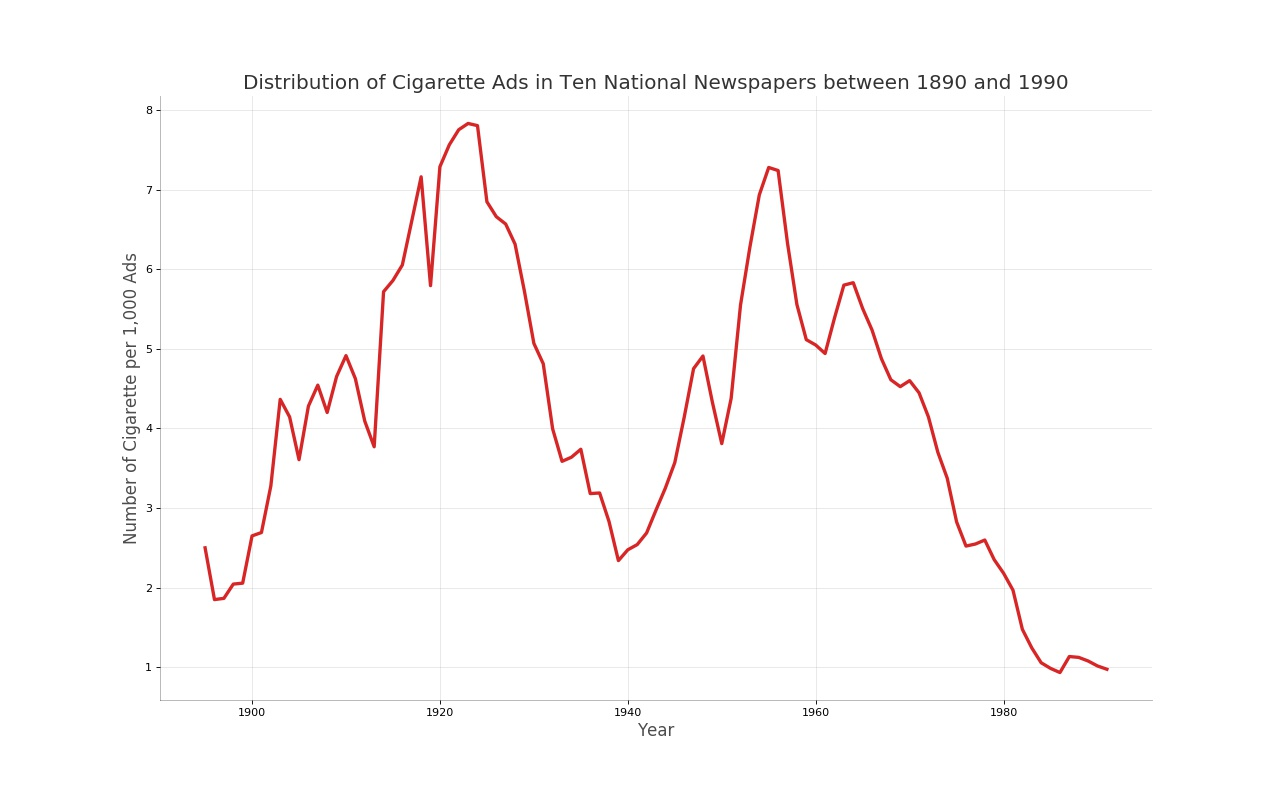
\includegraphics[width=.9\textwidth]{figures/cigarette_ads}%
  \caption{Relative Number of Cigarette Advertisements 1890-1990}%
  \label{fig:cigarette_ad_curve}%
\end{figure}

Plotting time series gives an overview of the temporal distribution of advertisements for a particular product. However, the search terms should be carefully selected. Using the different spelling variations, captured with the regular expression, this query covers most of the historical variations in the twentieth century. In the case of cigarettes, the decrease in the last quarter of the twentieth century can in part be explained by the fact that advertisers stopped referencing cigarettes explicitly. Rather, they turned to ads that include brand names or logos but not 'cigarette'. In such instances, computer vision could help to detect cigarettes or the occurrence of particular logos in advertisements. Many of these brand names are ambiguous, and querying them could also return advertisements for unrelated products. 
%
Moreover, the period during the Second World War should also be scrutinized more closely, since only a few newspapers were published throughout this period, and the size and content of newspapers transformed drastically. Even when using relative frequencies to offset the changing number of newspapers, we cannot account for such factors. 

\subsection{Cigarettes and Product Nationalities}
While text mining allows to study of large-scale trends, it can also help to explore more specific ways in which advertisers framed a product. One type of framing is the nationality of a consumer good, also known as product nationality. The relationship between products and constructions of nationality has long since been debated in consumer and marketing studies~\cite{thakor_brand_1996, hull_cultural_2016}. A key finding in these studies is that a strong connection to a favored country persuades consumers to spend more money on products with such a connection~\cite{menapace_consumers_2011}. The representations of product nationality are more than mere associations, they are ``powerful narratives about the meanings and values transferred by products from their origin to their destination~\cite{askegaard_product-country_1998}.''

In the case of the cigarette, the representation of product nationalities is an under-researched topic, which is surprising given that advertisers explicitly connected cigarettes to particular countries and regions.  These product nationalities referred to their actual or perceived country of origin, but often they also communicated particular characteristics associated with these countries. 

\begin{figure}
  \centering
  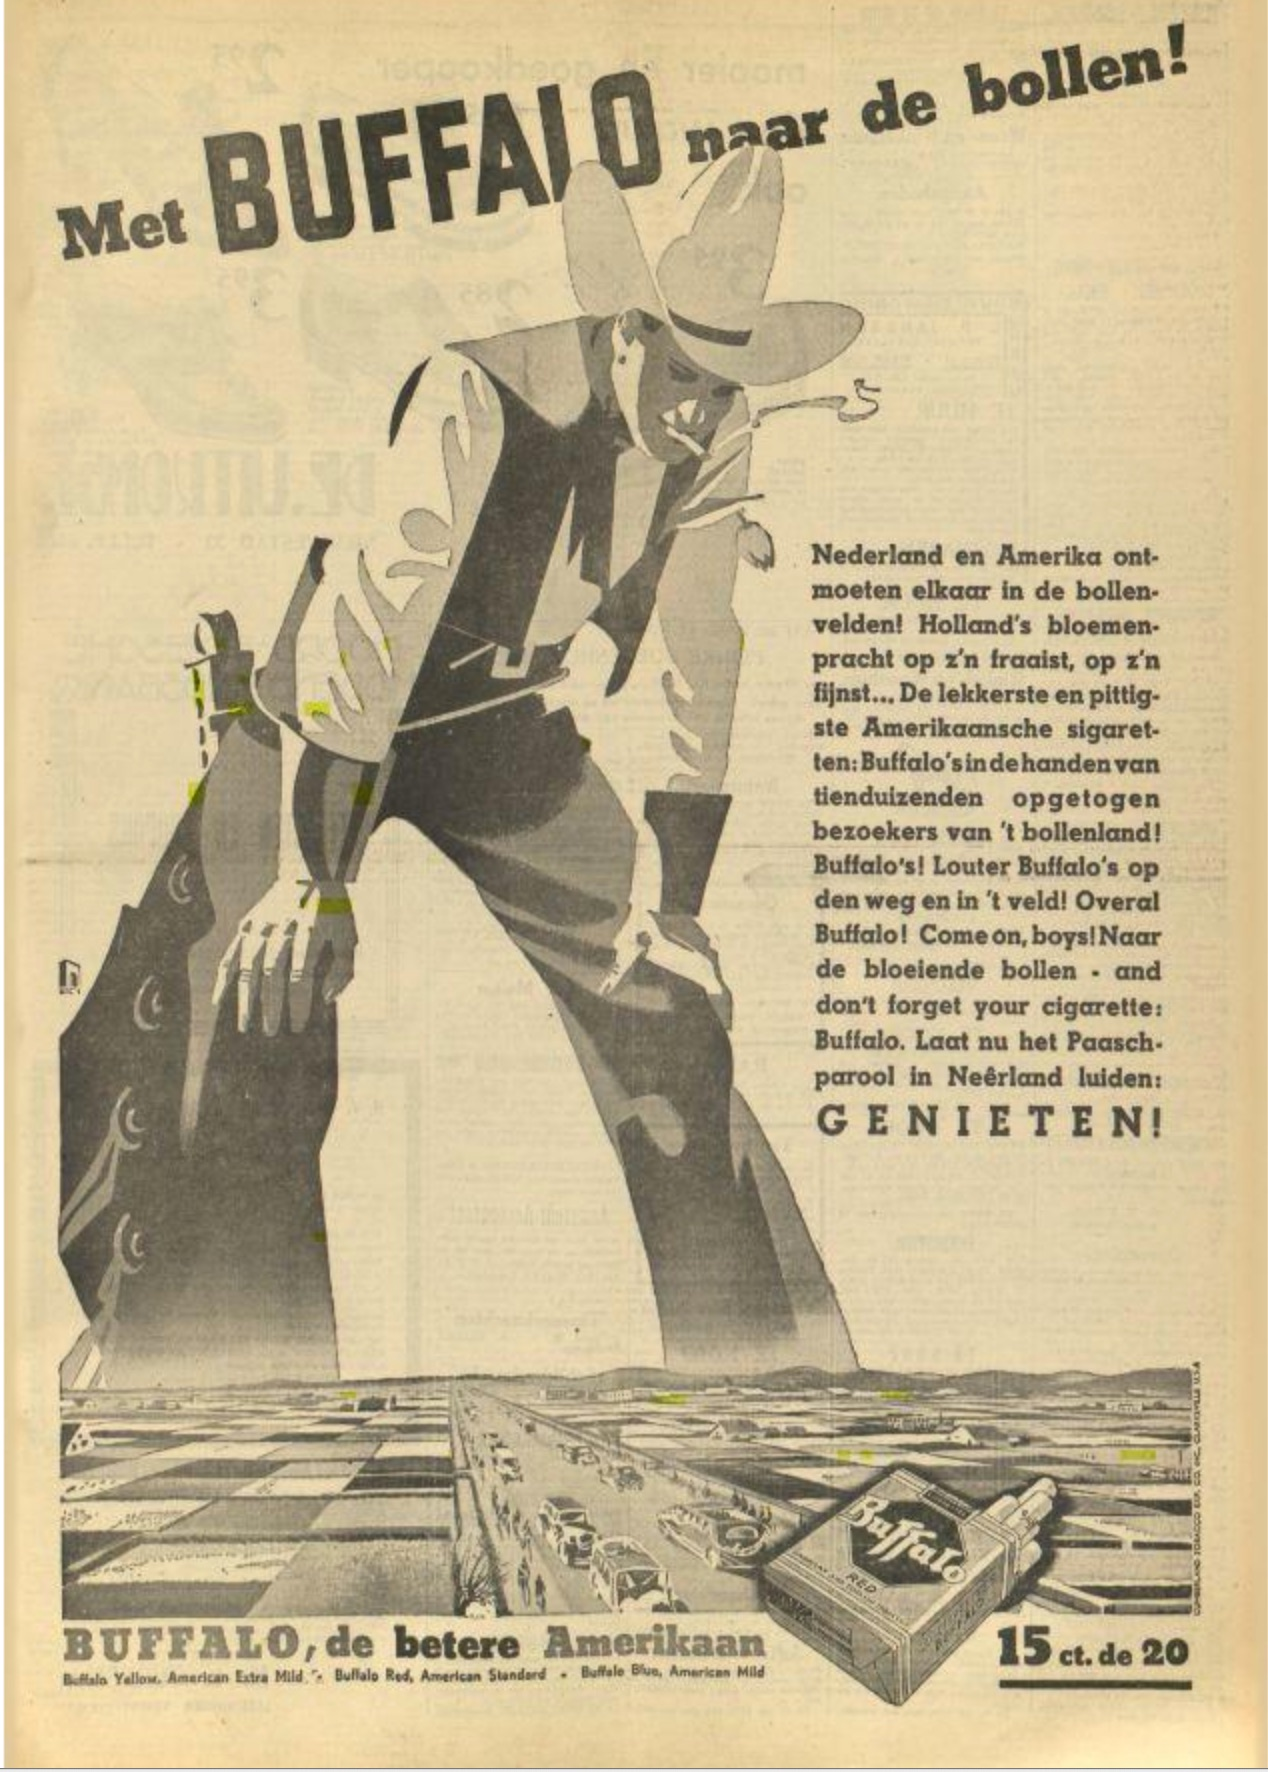
\includegraphics[width=.9\textwidth]{figures/example_buffalo.jpg}
  \caption{Advertisements for Buffalo cigarettes in \textit{Limburger Koerier}, April 13, 1938}
  \label{fig:buffalo_example}
\end{figure}

The advertisement in Figure~\ref{fig:buffalo_example} is a clear example of the association between product nationality and particular characteristics. This  1938 advert for the Buffalo cigarette linked the brand to the United States in several ways. First, the brand's name Buffalo denoted the emblematic American prairie animal as well as the city of Buffalo in upstate New York. The relationship between the brand and the United States was further enforced by a small print mentioning its producer: The Cumberland Company from Clarksville, USA.
%
Second, in addition to these textual cues, the advertisement included a visual signifier: a background image of a giant cowboy bending over a Dutch tulip field. This picture of a cowboy—an exemplar of American culture—further substantiated Buffalo as an American cigarette. Furthermore, this image expressed the towering dominance of American products in the Netherlands.
%
Third, the ad presented the Buffalo cigarette as having an American product nationality by describing it as ``the tastiest and spiciest American cigarette.'' The geographical association to the United States suggested the product’s country of origin, but also signified a particular taste specific to American techniques of tobacco preparation.

The Buffalo ad is of course just one example. How does this particular advertisement compare to others, and is its messaging specific to cigarettes with an American product nationality? Using text mining, we can gather the information that help us answer questions like these. 

\subsection{Charting Product Nationalities}
We can, for example, chart the nationalities most commonly associated with cigarettes in advertisements. There are two basic ways to establish product nationality. First, we could count the occurrence of bigrams---two adjacent word tokens---that include an explicit reference to nationality and cigarettes. For example, to find out when and how often advertisers described cigarettes as American, one could count the advertisements that contained bigrams such as American Cigarette (\textit{Amerikaanse sigaret}). Regular expressions can help to capture a wide range of possible spelling variations of such a bigram. However, a key flaw in counting the bigram 'American cigarette' is that we then only enumerate instances in which 'American' appeared directly to the left of cigarette. Advertisers, however, also used other ways to relate cigarettes to a particular location. For instance, in the case of Egyptian cigarettes, advertisers relied on phrases such as ``imported from Egypt.'' One possible yet time-consuming solution is to construct a list of all possible strings that express a relationship to a specific nationality. 

A second method is to count references to nationality that co-occurred in the  proximity of the word cigarette. In this approach, one only counts words that co-occur within a specific span of words, rather than advertisements that contain the two words. The co-occurrence of words in one advertisement does not necessarily indicate a relationship between them. 'American' could appear in an advertisement for cigarettes without referring to the product nationality of the cigarette or one of its features. Nevertheless, word proximity is a good indicator of a semantic relationship between the given words. Hence, in what follows, we count references to America within a span of five words to the right or left of the keyword 'cigarette'. 

One could also look for the co-occurrence of the two terms in one document without the use of a span. However, during digitization, the Optical Layout Recognition (OLR) did not always correctly compartmentalize advertisements. There are, for instance, cases where cigarette and America appeared in the actual newspapers in two separate advertisements, whereas after digitization, they were identified as one single advertisement (see Figure~\ref{fig:segmentation}). In Figure~\ref{fig:segmentation}, American refers to the American hotel in Amsterdam, and \textit{sigaretten} to an unassociated retailer advertising cigarettes. The words appeared in one single advertisement, albeit separated by a large number of words. Therefore, the use of a span of five words would not have counted this as an instance in which the two words appeared together. Looking for words in proximity to each other reduces the impact of errors produced by composite advertisements.

\begin{figure}%
  \centering
  %
  %\qquad
  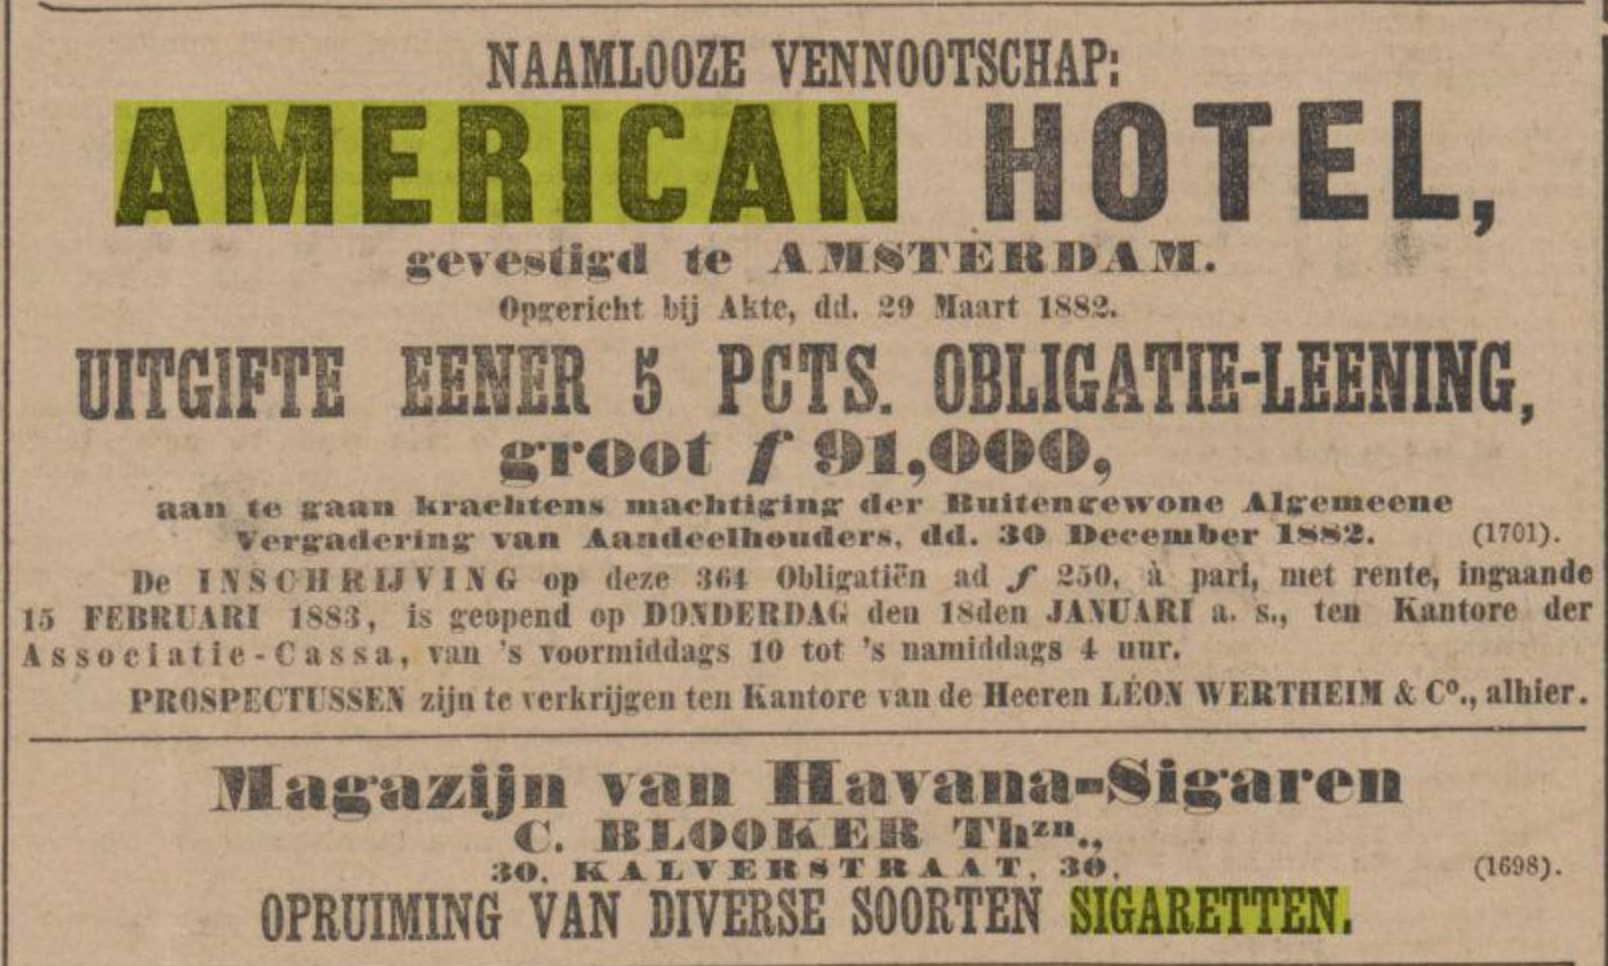
\includegraphics[width=.9\textwidth]{figures/segmentation_error}%
  \caption{Example of an incorrect segmentation of advertisements. \textit{Algemeen Handelsblad}, January 15, 1883}%
  \label{fig:segmentation}%
\end{figure}

For this section, we charted six product nationalities associated with cigarettes: American, British, Egyptian, Russian, Turkish, and Virginia.\footnote{We approach Virginia as a nationality, since the term came to represent Britain} Using regular expressions, we queried the singular and plural variants of these references as well as common spelling variations. The occurrence of these words in advertisements serves as a proxy for the popularity of cigarettes with varying product nationalities. Figure~\ref{fig:cig_nationality} shows the relative frequency of references to nationalities per 1,000 cigarette advertisements. 

\begin{figure}%
  \centering
  %
  %\qquad
  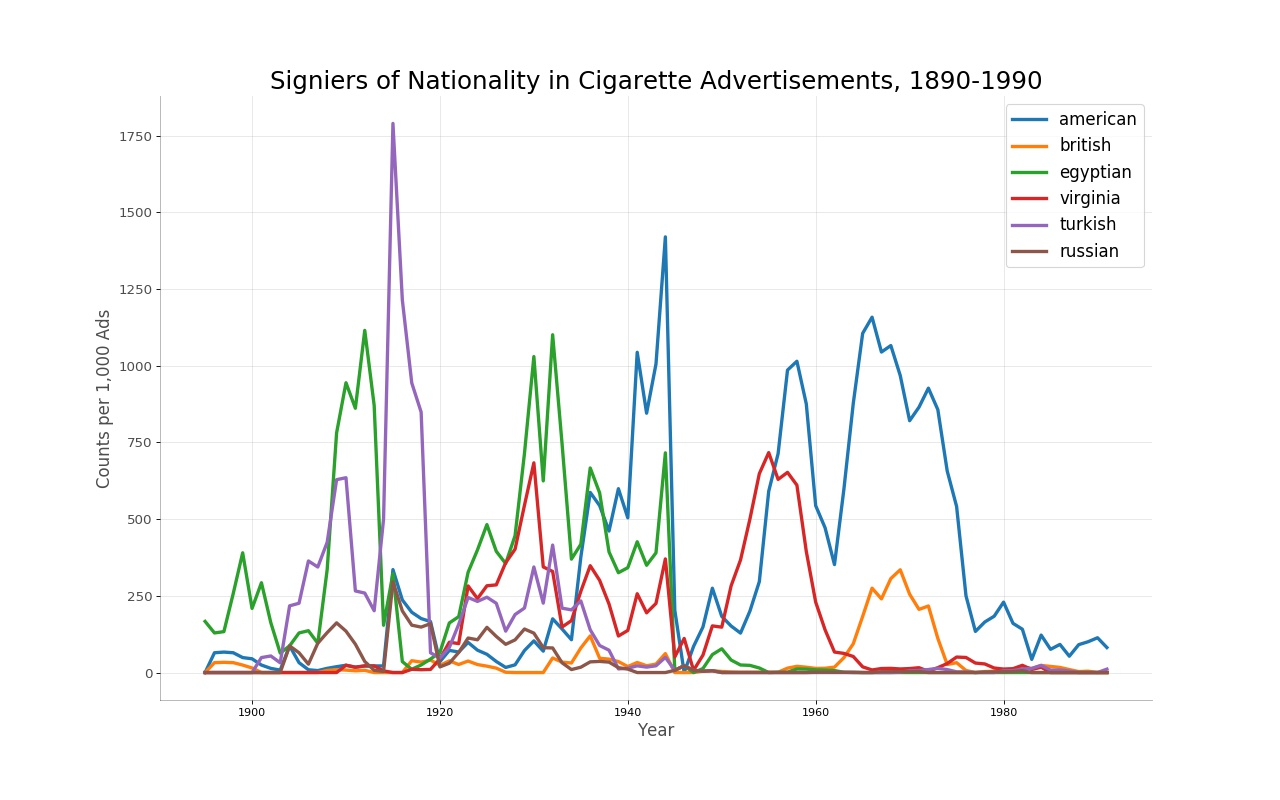
\includegraphics[width=.9\textwidth]{figures/cigarette_nationality}%
  \caption{Relative frequency of signifiers of nationality in cigarette advertisements, 1890-1990}%
  \label{fig:cig_nationality}%
\end{figure}
 

From 1890 to 1919, Egyptian, Turkish, and Russian cigarettes were the most popular. The popularity of these cigarettes mirrored the economic, cultural, and political power of the associated geopolitical entities. Before the First World War, the popularity of Russian and Turkish cigarettes mirrored the might of the Ottoman and Russian Empires. In the same period, the American cigarette industry was making its first forays into the European cigarette market~\cite{brandt_cigarette_2009}.
%
Right after the First World War, Virginia and Egyptian cigarettes became the most popular cigarettes. After the First World War, the British cigarette industry, and especially British American Tobacco (BATCO), played a prominent role in the production and distribution of both Egyptian and Virginia cigarettes~\cite[27-8]{shechter_smoking_2006}. BATCO was also instrumental in disseminating Virginia cigarettes in the Netherlands.

The association with the United States gained prominence after the Second World War, when both American and Virginia cigarettes towered above the other nationalities, which by that time had disappeared almost entirely. In the 1960s, when Virginia cigarettes lost their popularity, the American cigarette acquired sole dominance. A decrease in references to the United States characterized the subsequent decades.
%
This decline coincided with the growing sentiments of anti-Americanism in the Netherlands~\cite{kroes_european_2006,gienow-hecht_always_2006}. Amid anti-American sentiments, advertisers might have refrained from associating their product with the United States. Furthermore, in 1964, the American Surgeon General Luther Terry published the Report on Smoking and Health in which he presented the detrimental effects smoking could have on one’s health. The report led to a significant decrease in cigarette consumption in the Netherlands and the United States \cite{hoffmann_less_2001}.

As this section has shown, counting specific strings of text in digitized material is a relatively easy and fast way to gauge and compare the popularity of particular products. The trends in popularity in Dutch newspapers matched global trends. However, the interest in American cigarettes already waxed before the Second World War, while academic literature on Americanization in the Netherlands commonly situates this process after the Second World War.

A next step could be to examine how particular products were presented in advertisements. In other words, were there distinct product features for cigarettes with particular product nationalities? Understanding the historical use of product features in advertising discourse can help us determine the cultural and technological impact of such products. 

\subsection{Product features}
In this section, we discuss two methods to examine the historical evolution of particular characteristics associated with cigarettes. First, we show how an algorithm to detect bursty word use can be leveraged to extract features that typified a certain period. Second, we demonstrate how machine learning can  determine whether cigarettes with a clear product nationality possessed  features distinct from cigarettes with other nationalities. 

\subsubsection{Finding Trending Topics using Burst Detection}
When we want to study the use of particular words and examine how this use has evolved, one of the first tasks is to decide which words we are actually studying? One method is to rely on secondary sources to construct a vocabulary of words related to a subject or particular period. A different approach is a data-driven one, in which we extract words that exhibit noteworthy use in the corpus using algorithms. One such algorithm is burst detection.

Burst detection is a modeling technique to detect \textit{bursts of activity} in streams of data, for example, the sudden rise and fall in word frequency in serial publications. The trends for individual words cannot just be compared. For example, for words with relatively little overall activity, a sudden, repetitive increase in use can signal a burst, whereas, for words with much activity, a different burst intensity might be required. Moreover, bursts of activity can also be nested within larger patterns. To be able to capture these bursts, Jon Kleinberg developed an algorithm that models the stream of information as an infinite-state automaton. The algorithm assigns costs to state transitions, which makes it possible to distinguish between short bursts and long burst even while the overall rate of transmission changes over time~\cite{kleinberg_bursty_2002}. We use Kleinberg's algorithm to detect whether and when specific words exhibited ``bursty'' behavior in advertising discourse. In other words, we use it to identify \textit{trending topics} in advertising discourse. 

We model the burstiness for a subset of words. This subset includes the 500 most distinctive, determined using tf-idf, adjectives and nouns from the corpus of cigarette advertisements. We then apply Kleinberg's algorithm using the default settings on monthly frequency counts of these 500 words. For each of these words, we get information on whether they bursted and how intense the burst was, as well as the duration of the burst. Figure~\ref{fig:burst_words} displays the top 50 bursty nouns and adjectives and when they bursted. We can  see the appearance of the key term filter around 1965 when the Surgeon General report also appeared. 

Moreover, the debate in the late 60s and early 1970s shifted toward the amount of nicotine in cigarettes. The appearance of the term health (\textit{gezondheid} in the mid 1920s stems from advertisements that promoted the health benefits of smoking Virginia cigarettes. The figure also contains phrases such as 'job application' (\textit{sollicitatie}) and 'human resources' (\textit{personeelszaken}). Upon closer inspection, these words appeared in job ads placed by cigarette companies, a category that researchers might want to prune from their corpus.

\begin{figure}%
  \centering
  %
  %\qquad
  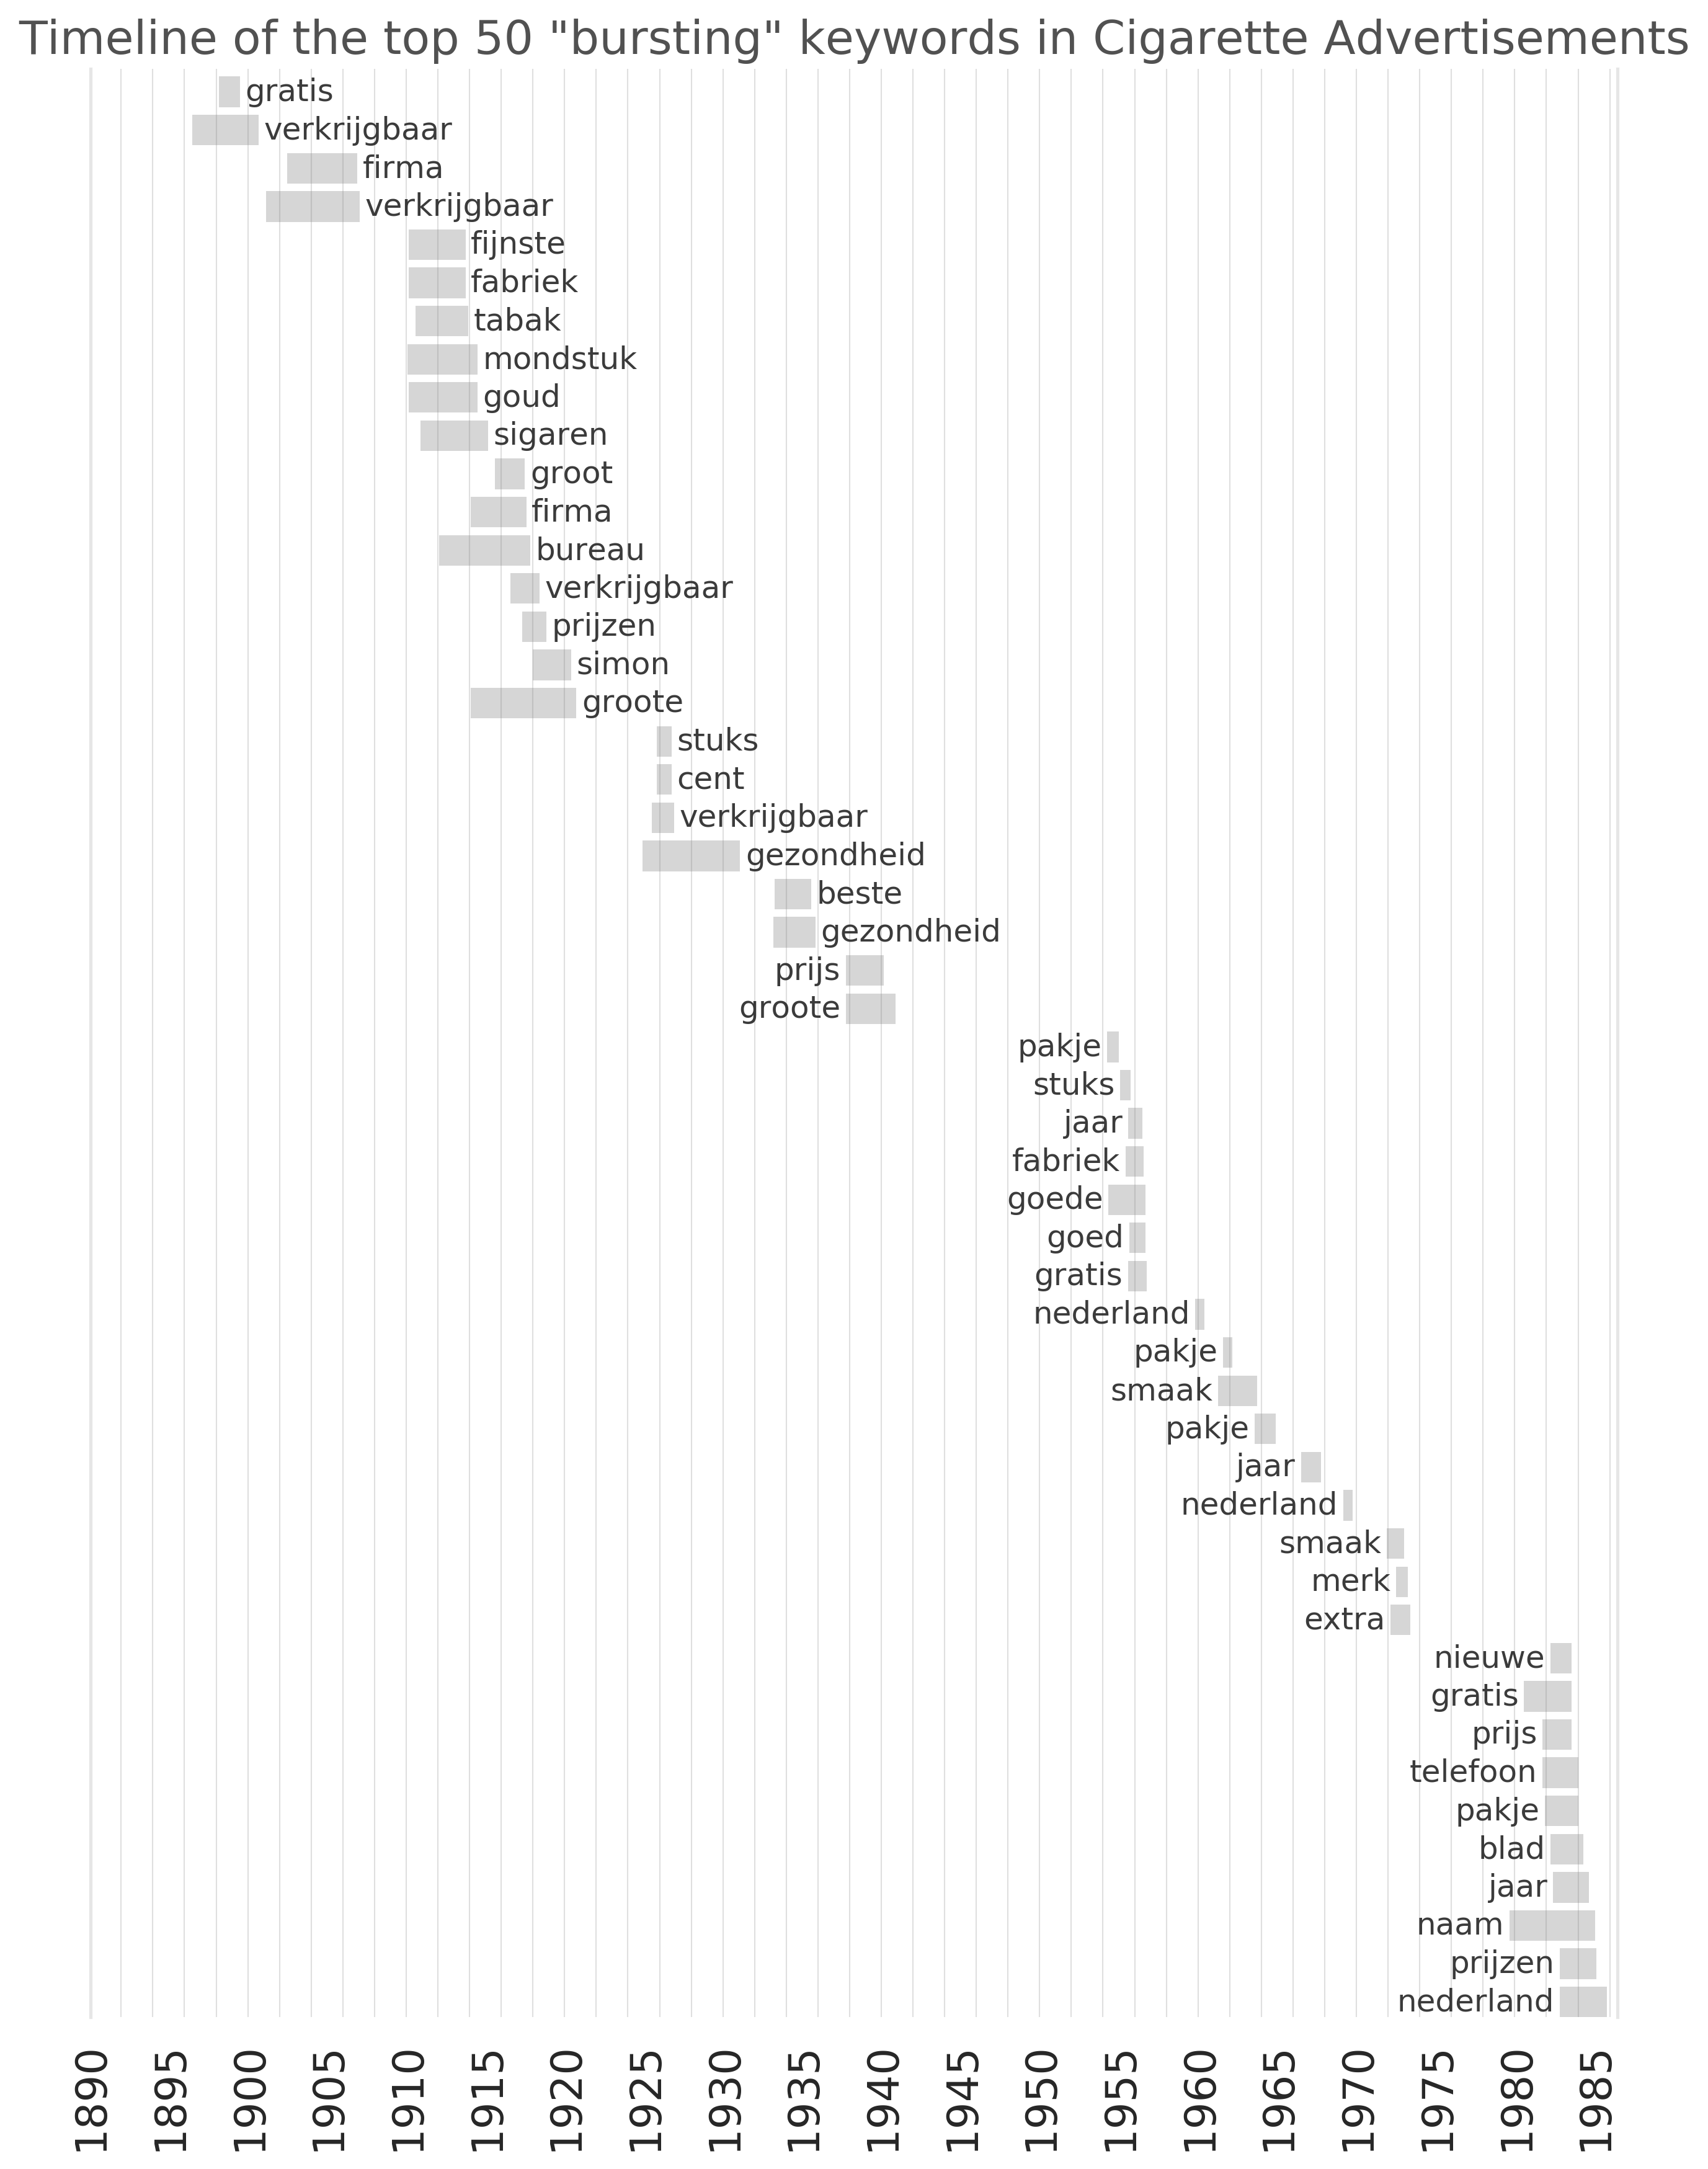
\includegraphics[width=.9\textwidth]{figures/bursts_top50}%
  \caption{Top 50 Bursty Nouns and Adjectives in Cigarette advertisements, 1890-1990}%
  \label{fig:burst_words}%
\end{figure}

Using this method, we can quickly gauge when particular words displayed ``bursty' behavior or which topics were trending at particular moments in time. This information can subsequently be used for closer examination of the texts in which these words appeared. Such techniques can also help distinguish a particular subset of that one might want to remove or treat as a separate corpus. 

\subsubsection{Detecting Distinctive Features Using Text Classifiers}
A different line of questioning might focus on the differences in vocabulary between cigarettes with varying product nationalities. For example, were American cigarettes more commonly associated with a mild taste, and were Egyptian cigarettes presented as artisanal? 
%
One method to gauge the differences between corpora is through the use of a machine learning classifier. These classifiers learn which textual features are predictive of a certain class. For example, which words are indicative of American cigarettes and which for Virginia cigarettes. This method assumes that language use between the two stays separated over time. In other words, if features are first introduced in Virginia cigarettes and then co-opted by American cigarettes, it might be more challenging to use this feature to distinguish between the two. For this reason, we can also train classifiers for separate periods, given that we have enough data. If the classifiers fail to separate the corpora, we can infer that the differences between language use were not very large. For each of these periods, we can also investigate the most informative features. 

We divide the corpus into subcorpora of ads that contain either references to the United States or to Virginia and the United Kingdom. After removing explicit references to nationalities, we train a Naive Bayes Classifier on the two corpora. For the period 1920-1980, in which both types of cigarettes were represented, the classifier is able to distinguish between advertisements for American and Virginia cigarettes with an accuracy of: 0.88, and respective $F_{1}$-scores of .92 and 0.79.  

Subsequently, we can examine the most informative features for the classifier to label an ad as either American or Virginia. Noteworthy results include brand names such as Lucky Strike, Roxy and Camel for American cigarettes, and Derby and Chief Whip for Virginia cigarettes. Moreover, words such as cork (\textit{kurk}), mouth piece (\textit{mondstuk}), purity (\textit{zuiverheid}), and health (\textit{gezondheid}) were predictive for Virginia cigarettes, while connaisseurs (\textit{liefhebbers}), packages (\textit{pakjes}), filter, and smoking pleasure (\textit{rookgenot}) are all predictive of American cigarettes.

The Ardath Company was primarily responsible for connecting these aspects to Virginia cigarettes; the British cigarette manufacturer boasted that the purity of its Virginia tobacco led to a better tasting and healthier cigarette. This link was particularly strong in advertisements for the brand Chief Whip, which Ardath described as the ``zenith of purity. Together with the company Wills, Ardath distinguished the taste of Virginia cigarettes from that of American cigarettes. Ardath and Wills both denounced saucing and blending--—two key features of the American cigarettes—--and distanced themselves from American cigarettes in doing so. In 1925, Wills claimed that its Virginia cigarettes consisted of 100\% pure Virginia tobacco, without the addition of Greek, Indonesian, or Turkish tobaccos. In advertisements for Chief Whip, a doctor claimed that the cigarette was ``absolutely pure and free of all surrogates and sauces.'' Advertisers presented Chief Whip as a pure and unprocessed cigarette.

The features used by the classifier point to three distinctive material aspects of the American cigarette: its length, its filter tip, and its packaging. Two addition that American cigarette producers introduced after the Second World War. 
%
First, in the 1950s, the longer, king-size cigarette was introduced to Dutch consumers, after enjoying great success in the United States. Advertisers linked the increase in length to the United States to help familiarize the Dutch smoker with the longer cigarette. In a 1955 advertisements, the brand So Long referred to the United States in their explanation of a king size cigarette: ``In America, a cigarette longer than 85mm is called King Size.''\footnote{``So Long advertisement,'' \textit{Het Vrije Volk}, December 13, 1955.} Advertisers used the link with the United States to help acquaint Dutch consumers with the longer cigarettes.

The second significant change was the introduction of filter cigarettes. Amid growing health concerns in the United States, American cigarette manufacturers introduced the purportedly healthier filter cigarettes in the early fifties~\cite[244]{brandt_cigarette_2009}. In the context of American filter cigarettes, purity did not denote the unblended nature of cigarettes, but the purifying effects of filters. Advertisements claimed that a lengthy filter would lead to ``more and purer smoking.''\footnote{``Sir Richard advertisement,'' \textit{De Telegraaf}, January 5, 1962.} Filter cigarettes became hugely popular, and by the 1970s, almost ninety percent of the cigarette market consisted of filter cigarettes~\cite[244]{brandt_cigarette_2009}. 

Third, technological developments in the United States changed the look and
feel of cigarette packaging. These innovations offered advertisers new ways
to link the product to the United States. American companies were the
first to package cigarettes mechanically in plastic-wrapped cardboard
boxes. Until then, consumers bought cigarettes per piece and stored them
in less practical tin boxes. The new method of packaging not only referred
to the United States because of its origin, but it also carried cultural
connotations that resonated with American culture. Advertisers described
the packaging of the American cigarette as flat, practical, modern, famous, or fancy. 

The information gained through this method can be used for closer examinations of particular characteristics, as demonstrated above. A more in-depth analysis falls outside of the scope of this chapter.\footnote{see \cite{wevers_consuming_2017-1} for such an analysis}

\section{Conclusion}
Advertisements are a rich and varied source for the study of public discourse. This chapter showcases how we can apply computational methods to metadata information to learn more about advertising in the past. The ability to distinguish between different types of advertisements can help to streamline further inquiry. Moreover, based on a case study on product nationalities in cigarette advertisements, we showed how text mining can help to better understand the historical trajectories between products and particular nationalities. Also, we demonstrated how the analysis of bursty words and machine learning can help to identify trending topics and distinctive words in advertising discourse. While the text is often far from perfect in digitized newspapers, there is still much we can extract from this abudance of source material using computational methods. With the increasing amount of digitized newspapers collections in different countries, we can also expand our efforts to study advertisements in a transnational perspective.


\begin{acknowledgement}
The author acknowledges the National Library of the Netherlands (KB) for making its newspaper data available.

\end{acknowledgement}

\bibliographystyle{apalike}
\bibliography{bibliography}
\end{document}
